% Utiliser des sections et des subsections pour les différentes parties du document.
% Utiliser begin{figure} pour les images sans oublier les labels pour le référencement

\section{Présentation générale}

\subsection{Archétype}

Notre but est de réaliser un jeu stratégique au tour par tour semblable à Advance Wars


\begin{figure}[h]
    \centering
    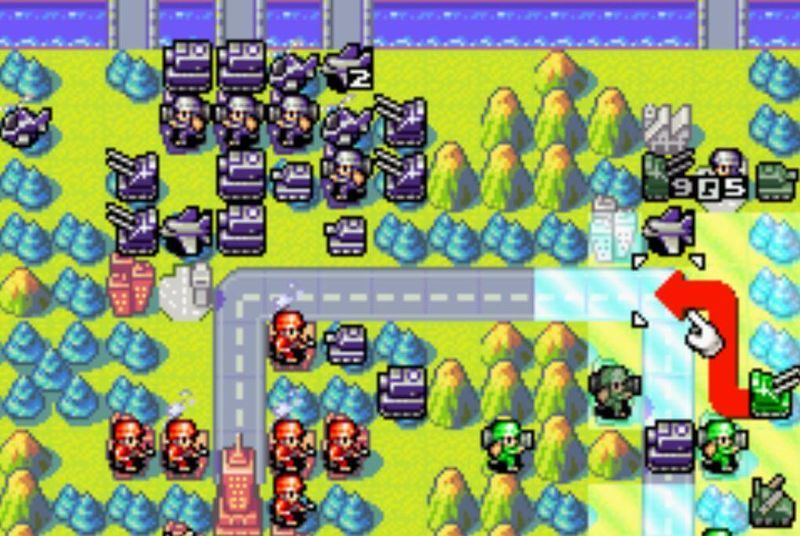
\includegraphics[scale = 0.5]{images/advanceWarsGameplay.jpg}
    \caption{Sprite des tuiles}
    \label{fig:Advance Wars}
\end{figure}


\subsection{Règles du jeu}

Notre jeu, "Until The Last Barrel", est un jeu de stratégie au tour par tour dont le but est de vaincre ses adversaires en capturant son Quartier Général (QG) sur le champ de bataille. Le dernier joueur survivant est donc déclaré vainqueur.
Pour se faire le joueur dispose de trois ressources: l'argent, le pétrole et des cartes.
\newpage

\subsubsection{Le champ de bataille}

Il s'agit d'une carte de tuiles (tile map) de différents types qui limitent ou améliorent la vitesse des unités des joueurs.
On peut notamment différencier les tuiles infranchissables comme les cours d'eau, et aussi les montagnes ou les forêts pour certaines unités, des plaines, chemins, routes et pont qui enjambent les cours d'eau.
Sur le champ de bataille se trouveront les QGs des joueurs, leurs unités, des villes, des usines et des puits de pétrole.



\paragraph{Les bâtiments}

Les bâtiments peuvent être capturés par les joueurs afin d'obtenir plus de ressources et autres avantages. Les puits de pétroles et les villes générent à chaque début de tour, respectivement du pétrol et de l'argent. Lorsqu'il veut jouer une carte le joueur peut placer des infanteries sur les villes et des unités motorisés sur les usines.



\subsubsection{Les ressources}

\paragraph{Les cartes}

Chaque joueur dispose d'un deck de carte duquel il pioche une carte à chaque début de tour. Une carte dispose d'un prix, qu'il est nécessaire de payer pour la jouer sur le champ de bataille, d'un type, de la description de ses effets. \n
\begin{itemize}
    \item \textbf{Les cartes unités} permettent pour un prix indiqué sur la carte d'invoquer sur le champ de bataille la dite unité. Dans le cadre des blindés, ceux-ci ne peuvent être invoqués qu'à proximité des usines.
    \item \textbf{Les cartes soutiens} se résolvent immédiatement sur n'importe quelle cible valide. Il peut s'agir d'un tir d'artillerie qui endommage des unités, à des soin ou encore de faire piocher le joueur.
    \item \textbf{Les cartes équipements} permettent d'améliorer les caractéristiques d'une unité alliée déjà présente sur le champ de bataille. 
    \item \textbf{Les cartes installations} sont un type de carte dont la fonction est de modifier les tuiles du champ de bataille. Il s'agit alors de pièges, bunker, pont, etc, afin de modifier le champ de bataille à son avantage. Les installations sont déployées à partir de certaines unités ayant la capacité nécessaire pour déployer l'installation voulue.

\end{itemize}


\paragraph{L'argent}

Au début de chaque tour, un joueur reçoit de l'argent en fonction de chaque ville qu'il a conquis, il peut alors dépenser cet argent lors de son tour afin de jouer des cartes. L'argent peut aussi être dépensé pour piocher des cartes.

\paragraph{Le pétrole}

Au début de chaque tour, un joueur reçoit du pétrole en fonction de chaque puit de pétrole qu'il possède, il peut alors utiliser ce pétrole pour déplacer des unités motorisées sur le champ de bataille. Si un joueur ne dispose pas de pétrole ces unités motorisées sont alors immobilisées voir détruites s'il s'agit d'unités aériennes.


\subsubsection{Les unités}
Il existe différentes unités jouables depuis sa main vers le champ de batailles avec différentes caractéristiques.\n 
De les unités de base ont : 
\begin{itemize}
    \item Des points de vie. L'unité est détruite si ses points de vie tombent à zéro.
    \item Des points de déplacement.
    \item Un niveau (conditionne les dégâts d'attaque par exemple).
    \item De la portée. Combien de tuiles peuvent être entre l'unité attaquante et l'unité attaquée.
    \item Des avantages face à certaines unités
    \item Des capacités spéciales
    \item Des équipements (ajoutés par d'autres cartes d'équipements)
\end{itemize}


\newpage
\subsection{Ressources}

Afin de pourvoir représenter les différentes unités, tuiles et autres éléments du jeu, nous avons crée par nous même des sprites. Nous utilisons une platte de 32 couleurs.

\begin{figure}[h]
    \centering
    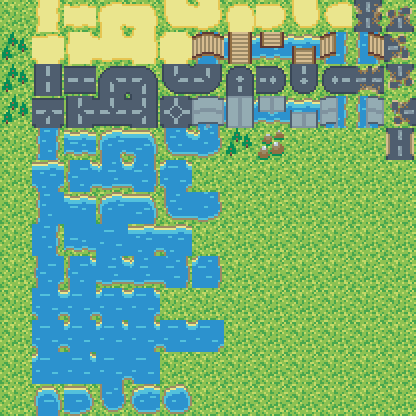
\includegraphics[scale = 1]{images/mapTileset.png}
    \caption{Sprite des tuiles}
    \label{fig:Advance Wars}
\end{figure}

\begin{figure}[h]
    \centering
    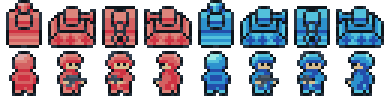
\includegraphics[scale = 1]{images/units.png}
    \caption{Sprite des unités}
    \label{fig:Advance Wars}
\end{figure}

\begin{figure}[h]
    \centering
    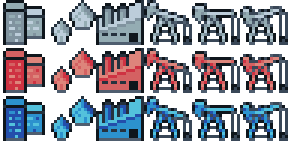
\includegraphics[scale = 1]{images/buildings.png}
    \caption{Sprite des bâtiments}
    \label{fig:Advance Wars}
\end{figure}

\clearpage

\section{Description et conception des états}

\subsection{Description des etats}

Un état du jeu est descrit par des éléments fixes (le champs de bataille), par un ensemble d'éléments mobiles (unités) et par les ressources des joueurs. Il existe aussi un compteur de tour afin de déterminer quel joueur peut jouer. On a donc:

\begin{itemize}
    \item Des coordonnées (x,y) pour les tuiles et les unités sur le champ de bataille
    \item Des classes différenciant les tuiles et les unités
    \item Des objets pour les joueurs déterminant les cartes, l'argent et le pétrole qu'ils possèdent.
    \item Un compteur pour les tours
\end{itemize}


\subsubsection{Eléments fixes}

Le champs de bataille est formé par une grille d'éléments nommé tuiles ou cases. La taille de la grille est fixée au démarrage de la partie. Les types de cases sont:

\begin{itemize}
    \item Les cases d'eau, de montagne et de forêt. Infranchissable par n'importe quelle unité.
    \item Les cases d'herbes qui permettent un déplacement standard.
    \item Les cases chemins qui permettent un déplacement plus rapide que celles d'herbe.
    \item Les cases routes qui permettent un déplacement plus rapide que celles d'herbe.
    \item Les ponts permettent de passer au dessus des cases d'eau et possèdent les mêmes caractéristiques que les chemins ou routes. Il existe.
    \item Les bâtiments se trouvent sur la carte. Ils peuvent soit être neutre, soit appartenir à un joueur. Parmis eux il existe: le QG, les usines, les villes et villages, et les puits de pétrole.
    \item Les installations sont des modifications du champs de bataille par les joueurs. Il peut s'agir de construire un pont, installer une barricade ou d'autres lignes de défence.
\end{itemize}

\newpage


\subsubsection{Eléments mobiles}
Les éléments mobiles autrement dit les unités possèdent une direction, un status fatigué, des points de mouvements, une position, des équipements, des PVs, un niveau, une spécialité. Les cartes sont elles aussi des éléments mobiles. En effet un joueur jouant une carte la fait passer de sa main au champs de bataille. \n
Il existe aussi des états intermédiaires quand le joueur décide de déplacer une unité ou jouer une carte.

\begin{itemize}
    \item Les points de mouvements autorise les déplacement selon le type de terrain. A zéro, l'unité est immobile.
    \item Le status "fatigué" (exhausted) pour savoir si l'unité peut entreprendre des actions ou non.
    \item Les PVs détermine si l'unité est en vie. A zéro l'unité est détruite et retirée du champs de bataille. 
    \item Le niveau est un état fixe qui détermine la puissance d'attaque de l'unité.
    \item Les équipements sont susceptibles de modifier les statistiques de l'unité équipé.
    
\end{itemize}


\subsubsection{Etat général}

Il existe quelques caractéristiques générales:

\begin{itemize}
    \item Un compteur de tour pour déterminer le joueur actif
    \item Un status "victoire" qui affiche au vainqueur et au vaincu la fin du jeu ainsi que son résultat.
    \item Une liste de joueurs ainsi qu'une liste des objets sur le champs de bataille.
\end{itemize}


\newpage


\begin{figure}[h]
    \centering
    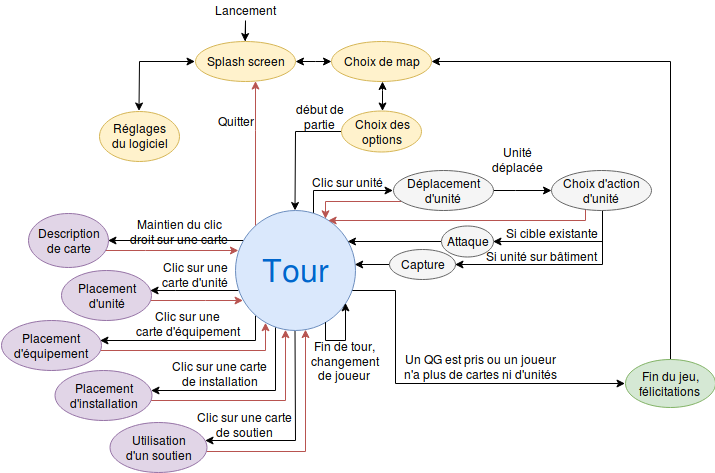
\includegraphics[scale =0.65]{images/etatsDeJeu.png}
    \caption{Diagramme du tour}
    \label{fig:Advance Wars}
\end{figure}


\begin{tabularx}{15 cm}{|X|X|}

\hline

\textbf{Description de l'état}  &  \textbf{Description de la transition} \\
\hline



\textbf{Splash screen} \newline Ecran d'acceuil & On peut accèder au \textbf{ Réglages du logiciel} ou au \textbf{Choix de map} grâce à un clic sur des icônes correspondantes \\
\hline
\textbf{Réglages logiciel} \newline Cela permettra de régler l'affichage et d'autres caractéristiques de la fenêtre & On peut retourner au \textbf{ Splash screen} via un clic sur un bouton retour. \\
\hline

\hline
\textbf{Choix de map} \newline C'est la liste des différentes maps concues que le joueur peut sélectionner. & On peut retourner au \textbf{ Splash screen} via un bouton retour ou arriver dans le \textbf{Choix des options} en confirmant son choix de map. \\
\hline
\textbf{Choix des options} \newline C'est ici qu'on peut régler différentes options comme la difficulté de l'IA etc... & On peut retourner au \textbf{ Choix de map } via un boutton retour, ou bien lancer la partie en commençant le premier \textbf{ Tour} \\
\hline
\textbf{Tour} \newline Le \textbf{Tour} permet à un joueur d'effectuer toutes les actions du jeu & 
Via la souris il peut: 
\newline -maintenir le clic droit pour avoir la \textbf{Description de carte} de l'une de celle qu'il a en main. Relâcher le clic fera revenir à l'état \textbf{Tour} précédent le clic.
\newline -avec le clic gauche sélectionner une de ses \textbf{Placement} (unité, équipement, installation) ou \textbf{Utilisation de soutien}, cette action peut être annulée par un clic droit. 
\newline -avec le clic gauche sélectionner une unité pour effectuer un \textbf{Déplacement d'unité} 
\newline -si le joueur adverse n'a plus de QG, la \textbf{Fin du jeu} est déclenchée.
\newline -la fin du tour qui voit un nouveau \textbf{Tour} se lancer avec un autre joueur aux commandes. \\


\hline
\textbf{Placement d'unité} \newline Suite à la sélection d'unte carte d'unité, le joueur peut décider de la faire jouer sur une case autorisée. & Un clic gauche sur une case autorisé fera apparaître l'unité de la carte sur le champs de bataille, et la carte sera alors défaussée. On retourne alors à \textbf{Tour}. \\
\hline

\textbf{Placement d'équipement} \newline Suite à la sélection d'unte carte d'équipement, le joueur peut décider de la faire jouer sur une unité autorisée. & Un clic gauche sur une unité autorisé fera apparaître l'équipement de la carte dans les caractéristiques de l'unité, et la carte sera alors défaussée. On retourne alors à \textbf{Tour}. \\
\hline

\textbf{Placement d'installation} \newline Suite à la sélection d'unte carte d'installation, le joueur peut décider de la faire jouer sur une case autorisée. & Un clic gauche sur une case autorisé fera apparaître l'installation de la carte sur le champs de bataille, et la carte sera alors défaussée. On retourne alors à \textbf{Tour}. \\
\hline

\end{tabularx}

\begin{tabularx}{15 cm}{|X|X|}

\hline

\textbf{Utilisation de soutien} \newline Suite à la sélection d'unte carte de soutien, le joueur peut décider de la faire jouer sur une case ou une unité autorisée. & Un clic gauche sur l'entitée autorisé déclenchera l'effet de la carte sur le champs de bataille, et la carte sera alors défaussée. On retourne alors à \textbf{Tour}. \\

\hline
\textbf{Déplacement d'unité} \newline On a sélectionnée une unité dans le but de la déplacer. Les cases où elle pourra se déplacer en fonction de ses points de mouvements & Un clic gauche permettra à l'unité de se diriger vers la case sélectionnée. Une fois le déplacement effectué, l'unité pourra effectuer une action dans \textbf{Choix d'action d'unité} \\

\hline
\textbf{Choix d'action d'unité} \newline On a déplacé l'unité on souhaite maintenant qu'elle effectue une action dans le tour. & Un clic droit fera revenir à \textbf{Tour} et l'unité n'effectuera aucune action. Un clic gauche sur un bâtiment lancera la \textbf{Capture} si l'unité est sur un bâtiment ennemi. Un clic gauche sur une unité adverse à portée déclenchera une \textbf{Attaque}.\\

\hline
\textbf{Attaque} \newline Un combat est lancé entre l'unité attaquante et l'unité attaquée & Une fois la résolution des dégâts terminée, on reprends le \textbf{Tour} \\


\hline
\textbf{Capture} \newline Une unité a commencé à capturer un bâtiment adverse. & Une fois le siège mis en place, le \textbf{Tour} reprendra automatiquement. \\

\hline
\textbf{Fin du jeu} & Une fois Celle-ci déclenchée, on revient au \textbf{Choix de map}  \\

\hline

\end{tabularx}








\newpage
\phantom{Texte invisible parce que j'ai pas trouvé d'autre méthode pour mettre le tableau à la ligne.}

\begin{tabularx}{15 cm}{|X|X|}
\hline
\textbf{GameState} \newline A pour but de décrire l'état du jeu & Attributs: map, players, existingCards, turn \newline Méthodes: GameState, getMap, addPlayer, getPlayer, endTurn, getTurn, GenerateRessource, getPlayerTurnId\\ 
\hline
\textbf{FieldObject} \newline C'est la classe qui décrit tout les objets du champs de bataille: leur emplacement, l'image associée, le propriétaire et le type  & Attributs: position, sprite, owner, type \newline Méthodes: FieldObject, setOwner, getPosition, setPosition, setObjectType\\
\hline
\textbf{Building} \newline Un bâtiment peut être capturé par des unités afin qu'un joueur en prenne le contrôle & Attribut: health \newline Méthode: Building, captured\\
\hline
\textbf{ObjectType} \newline C'est une classe dénumération des types possibles que peut prendre un FieldObject & Attributs: HEADQUARTER, TOWN, FACTORY, OILWELL, INSTALLATION, UNIT \newline \\
\hline
\textbf{Headquarter} & Attribut: moneyProduction \newline Méthodes: Headquarter, setMoneyProduction, captured, setMoneyProduction, getMoneyProduction\\
\hline
\textbf{Town} & Attribut: moneyProduction \newline Méthode:Town, Town (un deuxième constructeur), setMoneyProduction, setMoneyProduction, getMoneyProduction\\
\hline
\textbf{Factory} &  
\newline\\
\hline
\textbf{OilWell} & Attribut:oilProduction \newline Méthodes: OilWell, setOilProduction\\
\hline
\textbf{Installation} & Attribut: sourceCard \newline\\
\hline
\textbf{Unit} & Attributs: equipments, headcount, sourceCard, direction, lastUpdate \newline Méthodes:getHeadCount, move, attack, defence, capture, getDirection\\

\hline
\textbf{Direction} \newline C'est une classe d'énumation qui permettra de changer les sprites en fonction des mouvements des unités & Attributs: UP, RIGHT, DOWN, LEFT \newline \\
\hline

\end{tabularx}



\begin{tabularx}{15 cm}{|X|X|}
\hline
\textbf{Map} & Attributs: tileset, size, data  \newline Méthodes: Map, getSize, getdata, getTile, getTileset\\
\hline
\textbf{Tileset} & Attributs: tiles, ressourcePath, columns, tileSize, resourceSize  \newline Méthodes: Tileset, getTile, getResourcePath, getColumns, getTileheight, getTileSize, getTilePosition, getTileIntRect\\
\hline
\textbf{Tile} & Attributs: speed  \newline Méthodes: Tile, getSpeed\\
\hline
\textbf{Player} & Attributs: deck, hand, money, oil, name, ownedFieldObjects, id, count  \newline Méthodes: Player, InitPlayer,  getMoney, setMoney, getOil, setOil, getId, getName, addOwnedFieldObject, removeOwnedFieldObject, getOwnedFieldObject, getCount\\
\hline
\textbf{Deck} & Attributs: cards  \newline Méthodes: Deck, Deck (deuxième constructeurs), pull, remove\\
\hline
\textbf{Cards} & Attributs: cards  \newline Méthodes: Cards, getCard\\
\hline
\textbf{Card} & Attributs: id, title, cost, decription, type  \newline Méthodes: Card, Card (un deuxième constructeur), playCard\\
\hline
\textbf{CardType} \newline Classe d'énumération pour différencier les types de cartes & Attributs: UNIT, EQUIPMENT, INSTALLATION, SUPPORT  \newline \\
\hline
\textbf{EquipmentCard} & Attributs: level, strengths, headCount  \newline Méthodes: EquipmentCard, playCard\\
\hline
\textbf{UnitCard} & Attributs:level, unitType, strengths, movesByTurn, oilCost  \newline Méthodes: UnitCard, playCard\\
\hline
\textbf{InstallationCard} & Attributs: stopOpponent, damage, iterations \newline Méthodes: InstallationCard, playCard\\
\hline
\textbf{SupportCard} & Attributs: damage, heal, moneyLoss, moneyGain, oilLoss, oilGain  \newline Méthodes: SupportCard, playCard\\
\hline
\end{tabularx}

\newpage

\clearpage

\begin{figure}[h]
    \centering
    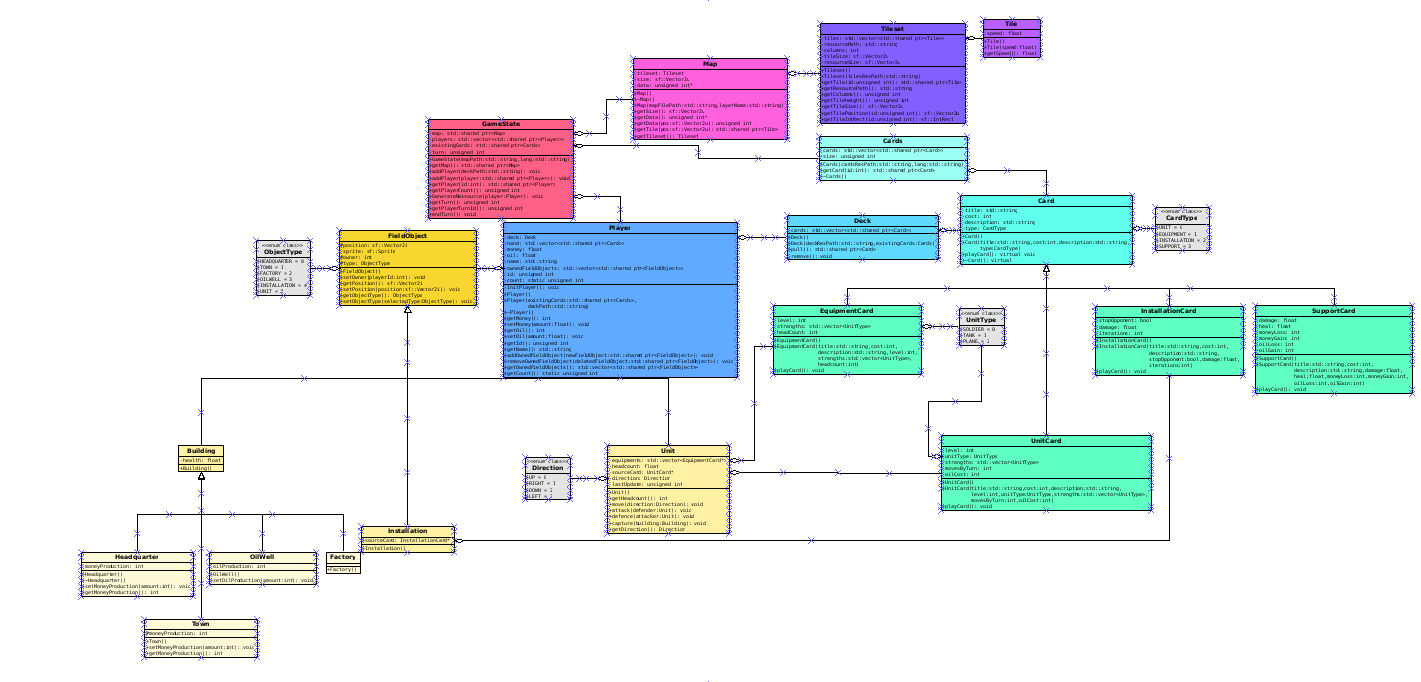
\includegraphics[angle=270,origin=c,scale =0.5]{images/state.png}
    \caption{Diagramme UML de l'état}
    \label{fig:Advance Wars}
\end{figure}

\clearpage

\section{L'affichage graphique}

\subsection{Premiers rendus}
L'affichage de la carte fonctionne grâce à l'implémentation d'un render. La carte est donc définie sous la forme de tileset dans le state, et importée dans le render afin de l'afficher.
Ainsi on constate qu'on a l'affichage dans une fenêtre de la carte ainsi que de fieldobject. 

\subsection{Descripteur de Tile}

Un affichage en bas à droite permet en lisant la position de la souris de donner les informations sur une case comme sa texture, son coût en déplacement et sa défense.

\begin{figure}[h]
    \centering
    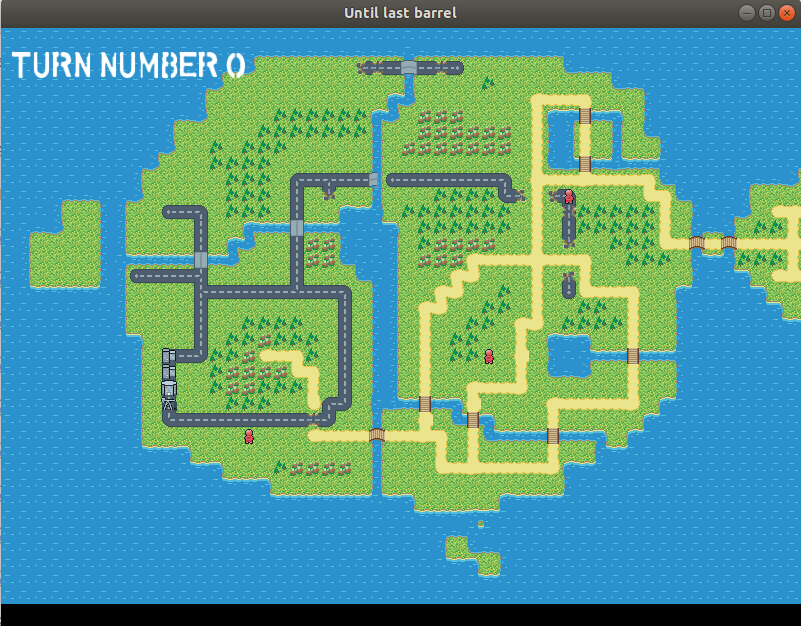
\includegraphics[angle=0,origin=c,scale =0.5]{images/demorender.png}
    \caption{Démonstration du render}
    \label{fig:Advance Wars}
\end{figure}

\newpage

\phantom{Texte invisible parce que j'ai pas trouvé d'autre méthode pour mettre le tableau à la ligne.}

\begin{tabularx}{15 cm}{|X|X|}
\hline
\textbf{Gstate} \newline A pour but de décrire l'état du jeu pour l'affichage & Attributs: gmap, gplayers, state \newline Méthodes: GState, getGmap, getGPlayers, getTurn, GePlayerCount,\\ 
\hline
\textbf{GRender} \newline C'est la classe qui décrit la fenêtre  & Attributs: window, cursor, cameraPosition, cameraZoom, armyFont, vcrFont \newline Méthodes: GRender, initTextures, getWindow, setCursor, display, getCameraPosition, updateCameraPostion, get CameraZoom, updateCameraZoom\\
\hline
\textbf{GPlayer} \newline Permet de déterminer quel objets de quels joueurs afficher & Attribut:  \newline Méthode: GPlayer, draw\\
\hline
\textbf{GMAP} \newline C'est une classe ayant pour but d'afficher la carte & Attributs: map
\newline Méthodes: GMap, draw, getTile, getTileDescription\\
\hline

\textbf{TextureManager} \newline Permet de gérer les textures & Attribut: textures, order \newline Méthode: TextureManager (constructeur et destructeur), getLength, GetTexture, loadTexture\\
\hline

\end{tabularx}

\newpage





\section{Le moteur}

Les mouvements ont été implémentés via un moteur. L'appui permet de modifier l'état en cours vers un nouvel état. En faisant ainsi on sépare l'affichage qui ne fait que lire, du moteur qui permet à la fois de lire l'état et de le modifier.


\subsection{Les commandes de jeu}

Il existe deux commandes afin d'agir sur le jeu: 
\begin{itemize}
    \item les commandes de direction qui permettent le mouvement des unités avec les touches directionnelles.
    \item Ctrl+Z permet d'annuler les déplacements du tour en cours.
    \item la commande de fin de tour avec la touche entrée.
\end{itemize}

\subsection{Les commandes d'affichage}
Pour modifier l'affichage de la carte ainsi que déplacer la vision du joueur, on peut utiliser le pad ou la souris.
\begin{itemize}
    \item L'aggrandissement de la carte est modifiable en étirant la fenêtre.
    \item shift+molette(scroll sur pad) permet de faire défiler la carte horizontalement.
    \item ctrl+molette (zoom sur pad) permet de zoomer ou dézoomer.
\end{itemize}


\newpage

\phantom{Texte invisible parce que j'ai pas trouvé d'autre méthode pour mettre le tableau à la ligne.}

\begin{tabularx}{15 cm}{|X|X|}
\hline
\textbf{GameEngine} \newline A pour but de gérer les commandes du joueur afin de modifier l'état du jeu & Attributs: currentState, commands, executedCommands \newline Méthodes: GameEngine(constructeur et desctructeur), getState, update, cancel, CancelFromPlayer, cancelTurn, addCommand, saveHistory, loadHistory\\ 
\hline
\textbf{Command} \newline C'est la classe qui décrit les commandes disponibles  & Attributs: playerTriggeringId, commandType (qui peut prendre deux valeurs 0 pour fin de tour et 1 pour les mouvements) \newline Méthodes: Command, execute, cancel, getPlayerTriggeringId, getCommandType, save\\
\hline
\textbf{CommandEndTurn} \newline Permet de finir le tour en cours & Attribut:  \newline Méthode: CommandEndTurn, execute, cancel, save\\
\hline
\textbf{CommandMove} \newline C'est une classe ayant pour but de commander les mouvement & Attributs: direction
\newline Méthodes: CommandMove, execute, cancel, save\\
\hline

\end{tabularx}

\newpage



\section{Les IA}

Deux types d'IA ont été crées.
La première euristique diminiue la distance de Manhattan avec les unités adverses sans tenir compte des obstacles.
La seconde essaiera que chacune de ses unités attaque les unités adverses les plus proches d'elles. 
\newline



\begin{tabularx}{15 cm}{|X|X|}
\hline
\textbf{CPU} \newline A pour but de gérer les IA pour générer les mouvements des joueurs non-humains & Attributs: state, engine, playerId, targetedPlayerId   \newline Méthodes: CPU, run\\ 
\hline
\textbf{RandomCPU} \newline C'est une IA dont les déplacements aléatoires & Attributs: playerTriggeringId,  \newline Méthodes: run, RandomCPU\\
\hline
\textbf{HeuristicCPU} \newline IA qui cherche à diminuer la distance de manhattan avec sa cible & Attribut: turnSteps \newline Méthode: run, HeurisitcCPU\\
\hline
\textbf{DeepCPU} \newline C'est une IA plus intelligente qui est capable de trouvé un chemin optimisé pour atteindre les unités adverses & 
\newline Méthodes: run, DeepCPU\\
\hline

\end{tabularx}





\section{Modularisation}

La mise en place de thread permet au moteur de fonctionner en parallèle du reste du jeu, notamment de l'affichage.
Le fichier replay.txt a été renommé pour devenir savefile.json.

\section{Progression}

Suite au développement nous avons décidé de ne pas implémenter la méchanique de carte pour le rendu final mais les fichiers nécessaire à sa création sont déjà présents.








